\section{Snow Simulator}

The snow simulator has been developed over several years by different students in 
the HPC-lab at NTNU as a part of their specialization project or master thesis. 
It simulates a finite number of snow particles and how they are affected by the 
wind and terrain. Here a short summary of the previous master theses and 
specialization projects that have worked on the snow simulator is given. This 
section also gives a short overview of the snow simulator and then goes into 
further details about the wind simulator.

\subsection{History}

The snow simulator was originally developed by Ingar Saltvik for his master
thesis \emph{"Parallel Methods for Real-Time Visualization of Snow"}
\cite{originalSnowThesis}. Saltvik's implementation was designed for multi-core
CPUs and achieved real-time performance for tens of thousands snow particles
and unknowns for the wind simulation. Figure \ref{fig:originalSnow} shows a 
screenshot of this snow simulator.

\begin{figure}[ht]
	\center
	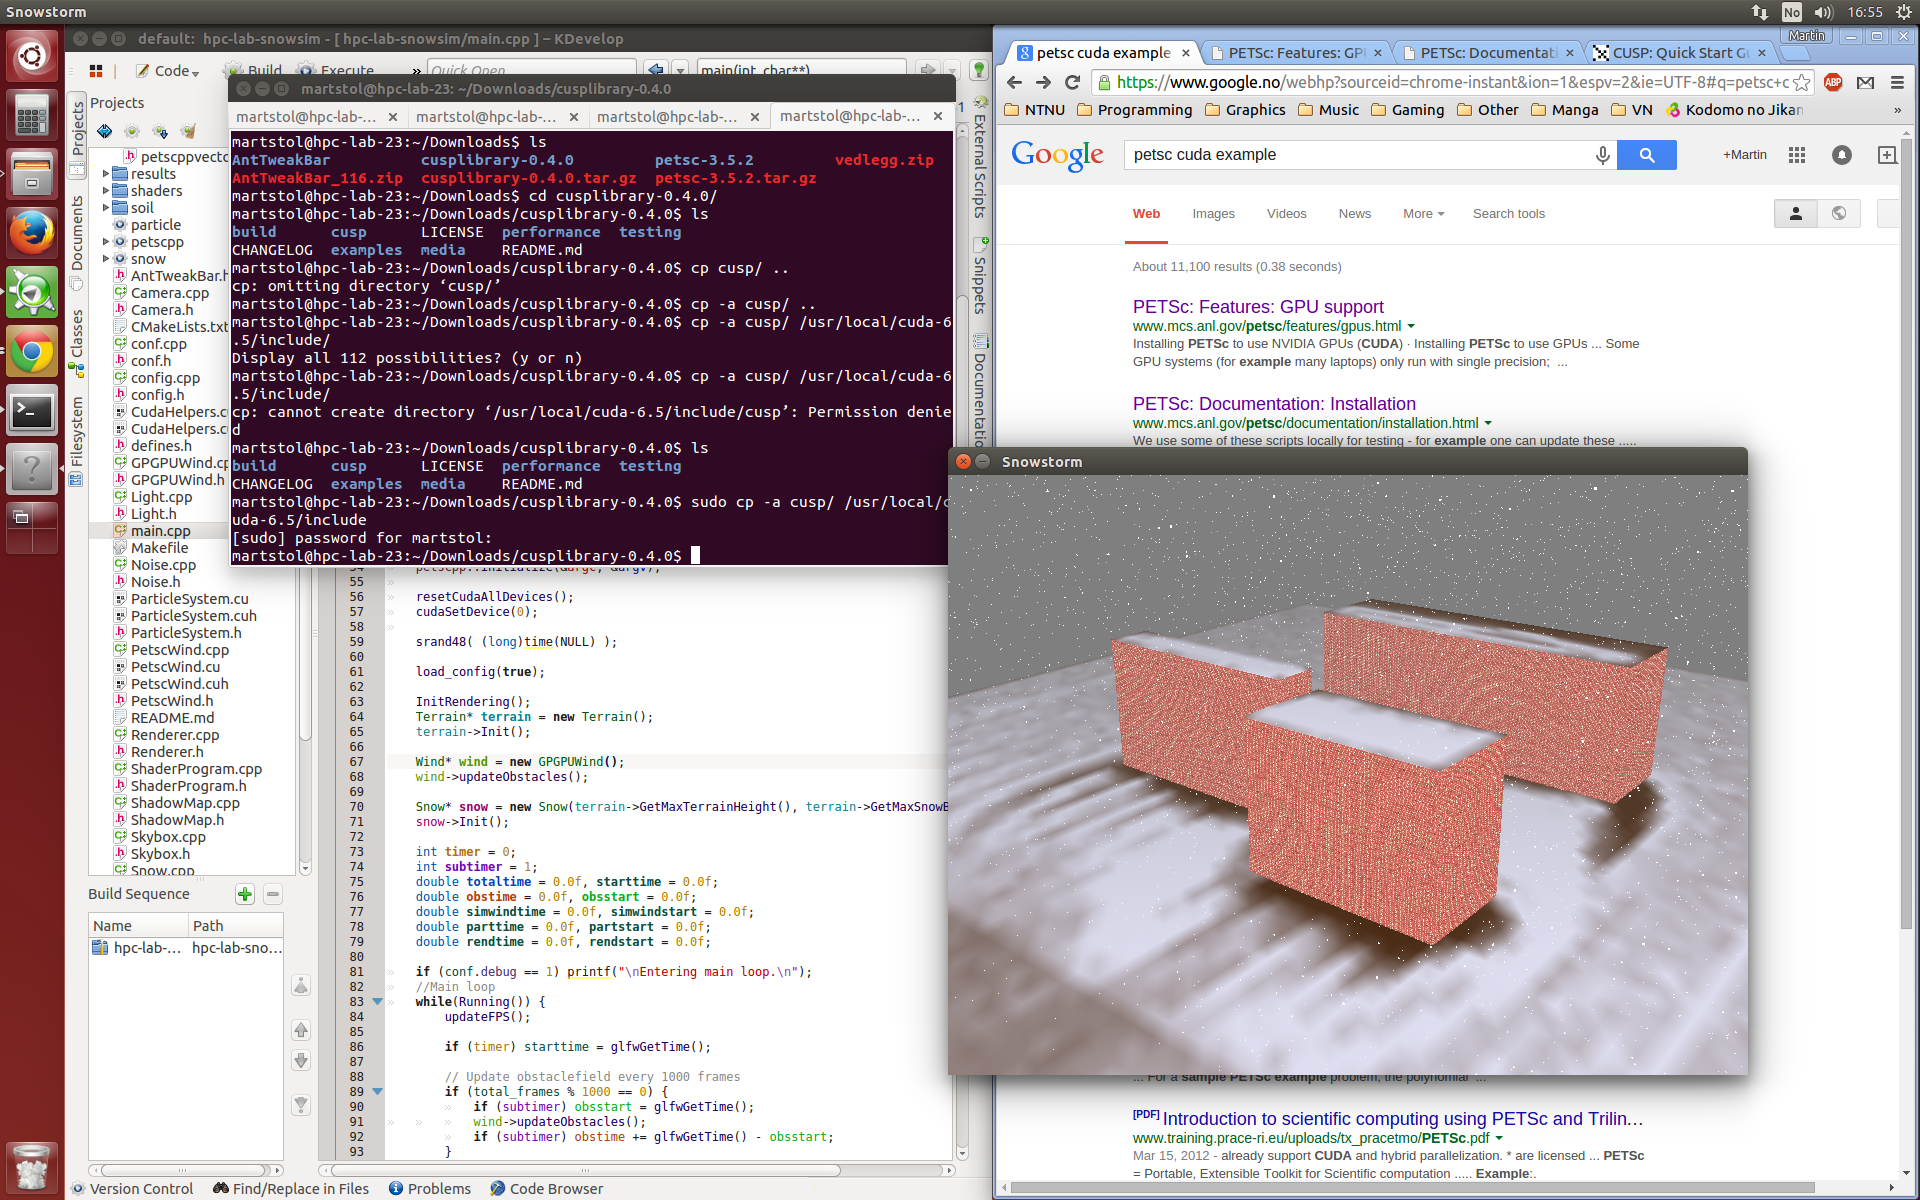
\includegraphics[width=1.0\textwidth]{images/snow/serial/snow5}
	\caption{The original snow simulator by Saltvik.}
	\label{fig:originalSnow}
\end{figure}

The snow simulator was later ported to the GPU using Nvidia's CUDA by Robin
Eidissen for his master thesis \emph{"Utilizing GPUs for Real-Time Visualization
of Snow"}\cite{gpuSnowThesis}. Eidissen's implementation achieved real-time
performance with more than two million snow particles and four million unknowns
in the wind simulation.

Alexander Gjermundsen\cite{lbmWind} compared the previously implemented
computational fluid dynamics solver with a solver using the Lattice Boltzmann
method and Joel Chellian\cite{fermi} improved this implementation by tuning it
for GPU's with Nvidia's Fermi architecture. Øystein Eklund Krog\cite{avalanche1}
implemented avalanche simulations into the snow simulator using smoothing
particle hydrodynamics on the GPU. Hallgeir Lien\cite{road} implemented a road
generation algorithm as a part of the snow simulator and a USGS DEM to RAW
height map converter, making it possible to use real-world maps in the snow
simulator. Frederik Magnus Johansen Vestre\cite{openclSnowThesis} ported the
snow simulator to GPUs designed for mobile phones and tablets using OpenCL and
compared the performance of the CPU and GPU when using OpenCL. Kjetil
Babington\cite{snowTerrainThesis} improved the terrain rendering and updated the
collision detection between the snow particles and the terrain. Andreas
Nordahl\cite{realisticSnowTerrainThesis} has improved the rendering of the snow
simulator by implementing several new visualization features. Magnus Alvestad
Mikalsen\cite{openAccThesis} ported the snow simulator to OpenACC and compared
the performance with the CUDA version. Øivind Laupstad Boge\cite{avalanche2}
implemented an avalanche simulator using fracture mechanics to calculate where
avalanches could occur.

The implementation of the snow simulator worked on during this project was rewritten 
by Magnus Alvestad Mikalsen and Andreas Nordahl for their specialization projects 
in an effort to improve the code base, which had been worked on by several other 
students\cite{openAccThesis}\cite{realisticSnowTerrainThesis}. 

\begin{figure}[ht]
	\center
	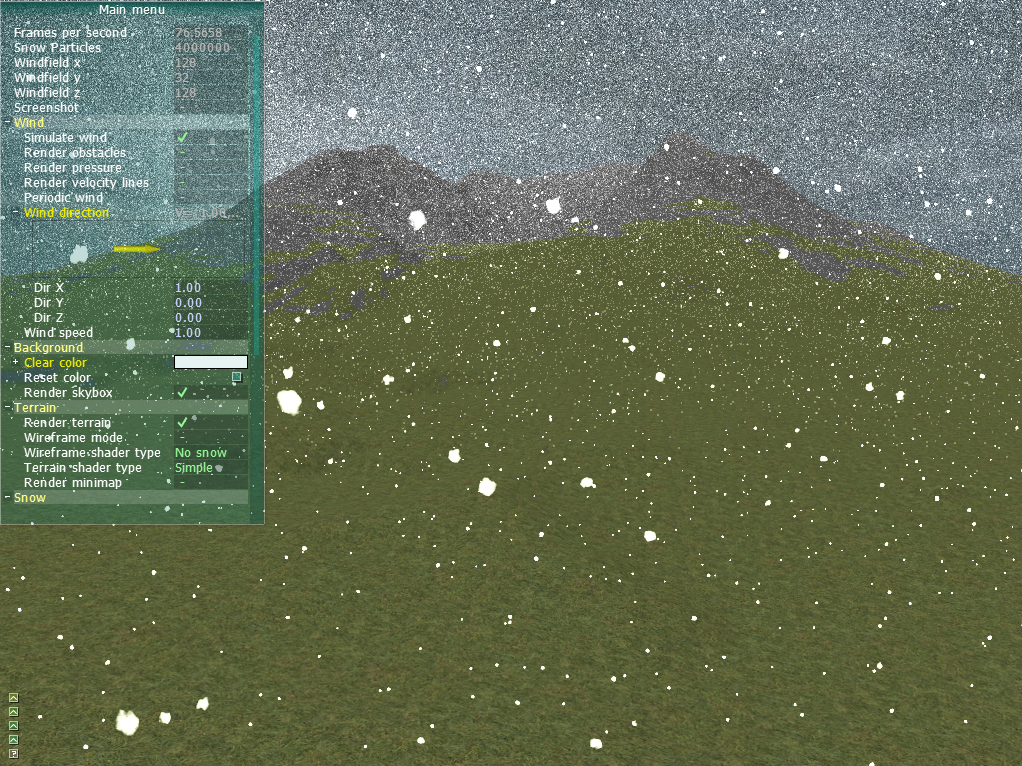
\includegraphics[width=1.0\textwidth]{images/snow/gpu/snow7}
	\caption{Current snow simulator implementation.}
	\label{fig:gpuSnow}
\end{figure}

\subsection{Overview}

The snow simulator is written in a combination of C, C++ and CUDA.
The four main components of the snow simulator is the \emph{wind simulator}, 
\emph{snow simulator}, \emph{terrain} and the \emph{renderer}. Figure \ref{fig:mainLoop} 
shows a short overview of the different stages in the simulation. 

\begin{figure}[ht]
	\center
	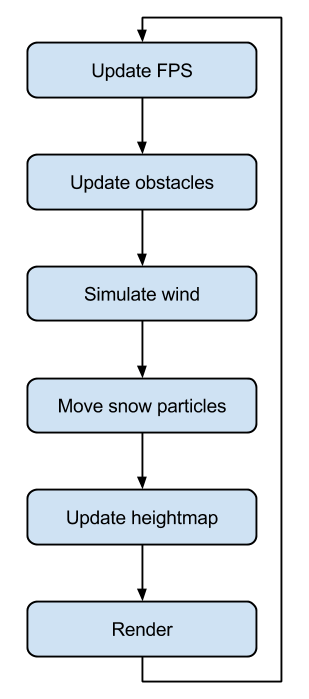
\includegraphics[width=0.30\textwidth]{images/snow_sim_main_loop}
	\caption{Snow simulator main loop.}
	\label{fig:mainLoop}
\end{figure}

The wind simulator solves the incompressible Euler equations to calculate the
wind velocity field. The wind simulator uses the terrain to create obstacles for
the wind. The snow simulator models the behavior of individual snowflakes as
particles with position, velocity and rotation. The snow simulator uses the
wind velocity field from the wind simulator to update the properties each
individual snow particle. When a snow particle lands on the ground it is added
to the terrain's height map.

The renderer uses OpenGL version 4.0 and shaders written in GLSL to make use of 
the programmable graphics pipeline. The renderer handles the windowing system, 
lighting, shadows, skybox, camera and user input. Rendering of the wind, snow and 
terrain is delegated to the corresponding component. The windowing system 
is GLFW\footnote{\url{http://www.glfw.org/}}, and GLEW\footnote{\url{http://glew.sourceforge.net/}} 
is used to get access to modern OpenGL functionality. 

\subsection{Wind Simulation}

The wind simulation calculates the three dimensional wind velocity field through
computational fluid dynamics (CFD). The discretization method being used is the
finite difference method. The boundary conditions for the CFD problem is decided
by the terrain vertex data and the external wind velocity at the borders of the
domain. The external wind velocity can be set by the user at runtime.

\subsubsection{Implementation}

The wind simulator is implemented in CUDA and consists of eight kernels. Five of 
the kernels are used for simulation while the remaining three kernels are for 
visualization. The wind simulation uses the following data structures:

\begin{description}
	\item[wind\_vel,] a three dimensional array of float4 representing the wind 
	velocity field. At the end of the wind simulation step, the contents of this 
	array is moved to texture memory for efficient access by the snow particle 
	simulation. 
	\item[obstacle,] a three dimensional array of integers. The bits of each 
	integer indicate if the current cell or an neighboring cell contains an 
	obstacle. 
	\item[pressure,] a three dimensional array of floats containing the values 
	of the air pressure used in the projection step of the wind simulator. 
	\item[solution,] a three dimensional array of floats containing the solution 
	vector (right-hand side) for the Poisson equation. 
\end{description}

Each of the five simulation kernels handles a part of solving the momentum equation 
of the incompressible Euler equations.
\begin{description}
	\item[wind\_advect]
	\item[build\_solution2]
	\item[solve\_poisson2]
	\item[set\_boundary2]
	\item[wind\_project2]
\end{description}

The visualization kernels are used to visualize the data structures used when 
simulating the wind. These are the visualization kernels:

\begin{description}
	\item[make\_obs\_points,] visualizes the cells determined to be obstacles 
	for the wind from the terrain. 
	\item[make\_pressure\_points,] creates color mapped points to visualizes the 
	pressure in the cells. 
	\item[make\_vel\_lines,] visualizes the wind velocity field as field lines 
	colormapped depending on the magnitude of the wind velocity vector. 
\end{description}

